%%%%%%%%%%%%%%%%%%%%%%%%%%%%%%%%%%%%%%%%%%

\chapter{Commissioning of the nEDM apparatus}\label{chap:nEDM_commissioning_dec2022}

%%%%%%%%%%%%%%%%%%%%%%%%%%%%%%%%%%%%%%%%%%

This chapter summarizes the first series of storage and spin asymmetry measurements obtained with the nEDM apparatus on the North beamline. 

%%%%%%%%%%%%%%%%%%%%%%%%%%%%%%%%%%%%%%%%%%

\section{Description of experimental setup (2022)}

%%%%%%%%%%%%%%%%%%%%%%%%%%%%%%%%%%%%%%%%%%

With the completion of the MSR (with the caveat of degaussing loop discontinuities, per Sec.~\ref{sec:MSR}), preparations were made for a December 2022 engineering run. The switchers and switcher stand (Chap.~\ref{chap:fall2021}) were moved from the West beamline and installed on the North beamline (Chap.~\ref{chap:north_beamline_paper}). The drop detector (Sec.~\ref{sec:spin_flipper_analyzer}) was mounted to the lower switcher, and the SSA (Sec.~\ref{sec:2021_experimental_setup}) was mounted to the upper switcher. Transport and $B_0$ coils were installed (Secs.~\ref{sec:B0_coil}, \ref{sec:transport_coils}). For magnetic field monitoring, two QuSpin Total-Field Magnetometers (Sec.~\ref{sec:magnetic_impurity_scanner}) and a prototype Twinleaf magnetometer (Sec.~\ref{sec:external_magnetometry}) were placed in proximity to the precession cells. Coils and solenoids applied to $\sim \qty{1}{mT}$ field to guides between the \acrshort{pm} and the MSR.

The central apparatus (Sec.~\ref{sec:precession_cells}), consisting of the glass-epoxy vacuum chamber, hydraulic cell valves, and two precession cells (dPS walls and NiP-coated electrode prototypes), was placed into the MSR. Guides between the switcher and the central apparatus comprised of polished Cu, and guides between the North GV and switchers were NiP-coated.

Due to irregularities on the vacuum chamber penetrations, the cell valve actuating arm was blocked from reaching the cell valve for the upper chamber, limiting measurements to only the lower chamber. The upper cell valve actuating arm was be redesigned after the measurement cycle. During the engineering run, the decision was made to exchange the Cu UCN guide connecting the upper switcher and upper chamber for a beam height UCN detector (Sec.~\ref{sec:2021_experimental_setup}).


%%%%%%%%%%%%%%%%%%%%%%%%%%%%%%%%%%%%%%%%%%

\section{UCN storage measurements}\label{sec:2022_ucn_storage_measurements}

%%%%%%%%%%%%%%%%%%%%%%%%%%%%%%%%%%%%%%%%%%

The fill and dump procedure (Sec.~\ref{subsec:holdingTimeMeasurement}) with a preload of \qty{100}{s} and a counting period of \qty{100}{s} was used for UCN storage in the lower cell. UCN counts in the drop detector were normalized to the average rate of the West GV monitor. Regardless of the filling period duration, the number of counted UCN after \qty{30}{s} of storage was only $\approx 600$ (Fig.~\ref{fig:2022_fill_time_sweep}).

The low number of stored UCN was still sufficient for a storage time measurement. The results are depicted in Fig.~\ref{fig:2022_ucn_storage}. The measurement was repeated for different configurations of the upper switcher orientation, where the upper switcher directed UCN from the wye to either a stainless steel blank-off or the beam height detector. The storage curves were fit with a single decaying exponential, yielding a storage time of $\approx \qty{30}{s}$

As a validation measurement, UCN were filled against a closed cell valve for \qty{50}{s}. (When the cell valve is closed, the UCN see a NiMo-coated surface.) The lower switcher was then turned such that \ucn between the closed cell valve and the switcher were emptied into the drop detector. This procedure would cause some UCN to be lost during the switcher actuation period ($\sim \qty{0.5}{s}$), but even without accounting for those losses the drop detector had a normalized count of $4350(65)$.

 \begin{figure}
    \centering
    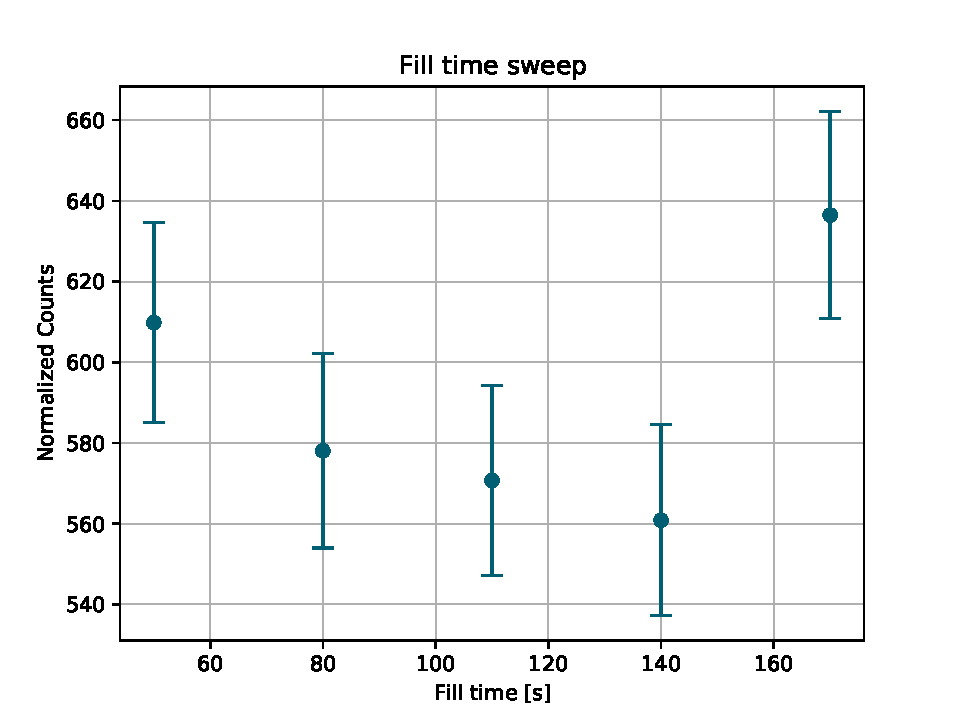
\includegraphics[width=0.6\textwidth]{figures/2022_fill_sweep.pdf}
    \caption
     {Fill-and-dump measurement in the 2022 nEDM apparatus. \qty{100}{s} preload with \qty{30}{s} storage. Counts are normalized to the average performance of the West GV monitor.}
    \label{fig:2022_fill_time_sweep}
\end{figure}


\begin{figure}
\centering
%subfigure width gets "multiplied" by includegraphics width
\begin{subfigure}{.5\textwidth} 
  \centering
  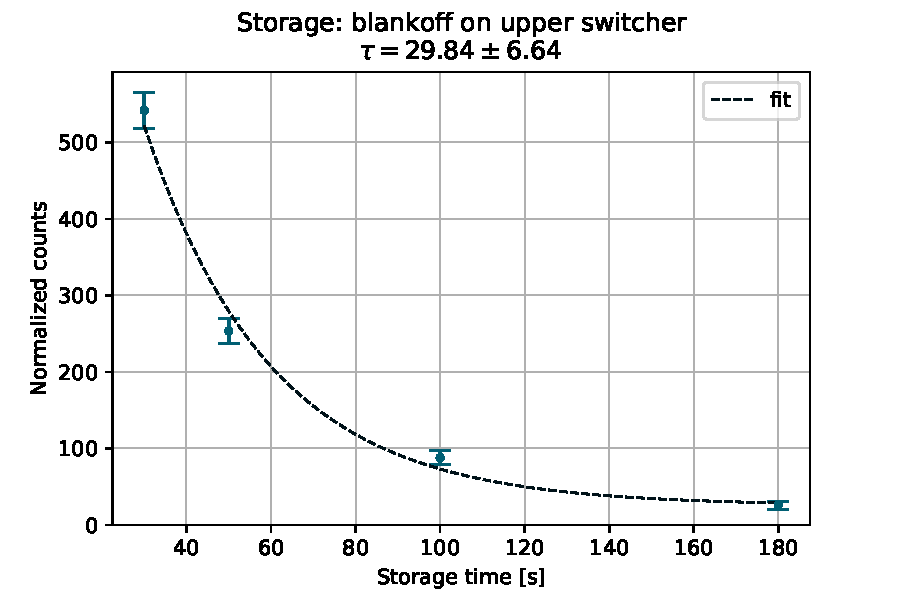
\includegraphics[width=\textwidth]{figures/store_blankoff_fit.pdf}
  \caption{}\label{subfig:2022_storage_blankoff}
\end{subfigure}%DO NOT REMOVE THIS '%'
\begin{subfigure}{.5\textwidth}
  \centering
  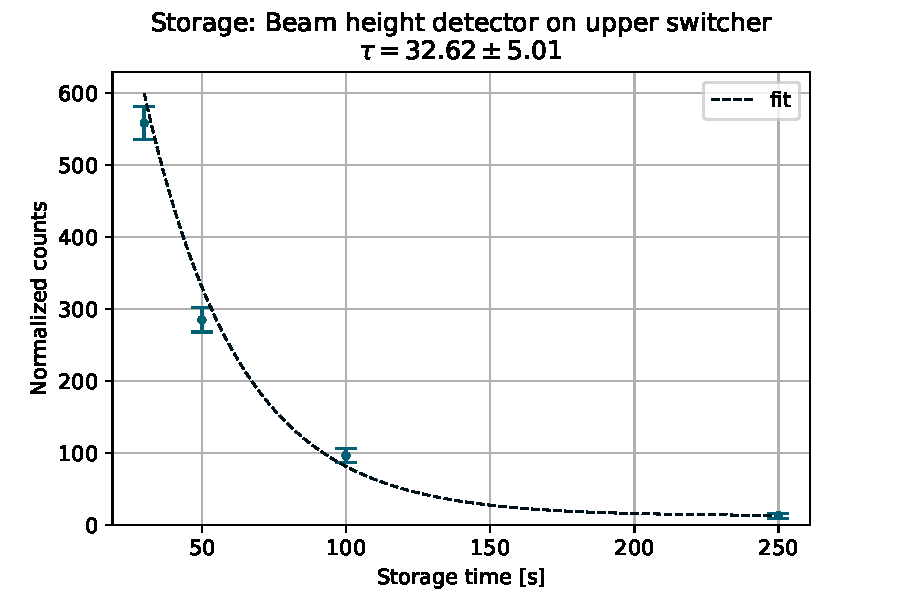
\includegraphics[width=\textwidth]{figures/store_with_beam_height_det_fit.pdf}
  \caption{}\label{subfig:2022_storage_beam_height_det}
\end{subfigure}
\caption
    [UCN storage time measurement in the lower precession cell of the apparatus fit with a single decaying exponential.]
    {UCN storage time measurement in the lower precession cell of the apparatus fit with a single decaying exponential. \textbf{(\subref{subfig:2022_storage_blankoff})} and \textbf{(\subref{subfig:2022_storage_beam_height_det})} differ in terms of where \ucn are directed on the upper switcher. \textbf{(\subref{subfig:2022_storage_blankoff})} terminates the upper switcher to a stainless steel blankoff, and \textbf{(\subref{subfig:2022_storage_beam_height_det})} terminates to a beam height \BZnS \ucn detector.}
\label{fig:2022_ucn_storage}
\end{figure}


%%%%%%%%%%%%%%%%%%%%%%%%%%%%%%%%%%%%%%%%%%

\subsection{Guide storage measurement}\label{sec:guide_storage_measurement}

%%%%%%%%%%%%%%%%%%%%%%%%%%%%%%%%%%%%%%%%%%

Encouraged by the increased UCN counts from the above validation measurement, a storage measurement was made using the Cu guides between the cell and switcher as the container. After the nominal \qty{100}{s} preload against the closed North GV, the lower switcher was placed in the filling position for \qty{50}{s} with the cell valve either open or closed. The switcher was then moved to the position illustrated in Fig.~\ref{subfig:2022_guide_storage_schematic}, which stored UCN in the guide volume between a SS blank-off on the switcher and the open/closed cell. For the counting period, the switcher was rotated to the position connecting the cell with the drop detector. The storage curve from the measurement with the cell valve closed (open) is depicted in Fig.~\ref{subfig:2022_guide_storage_cell_closed} (Fig.~\ref{subfig:2022_guide_storage_cell_open}). The upper switcher directed UCN from the wye to the steel blankoff for the entirety of the measurement.



\begin{figure}
\centering
%subfigure width gets "multiplied" by includegraphics width
\begin{subfigure}{.5\textwidth} 
  \centering
  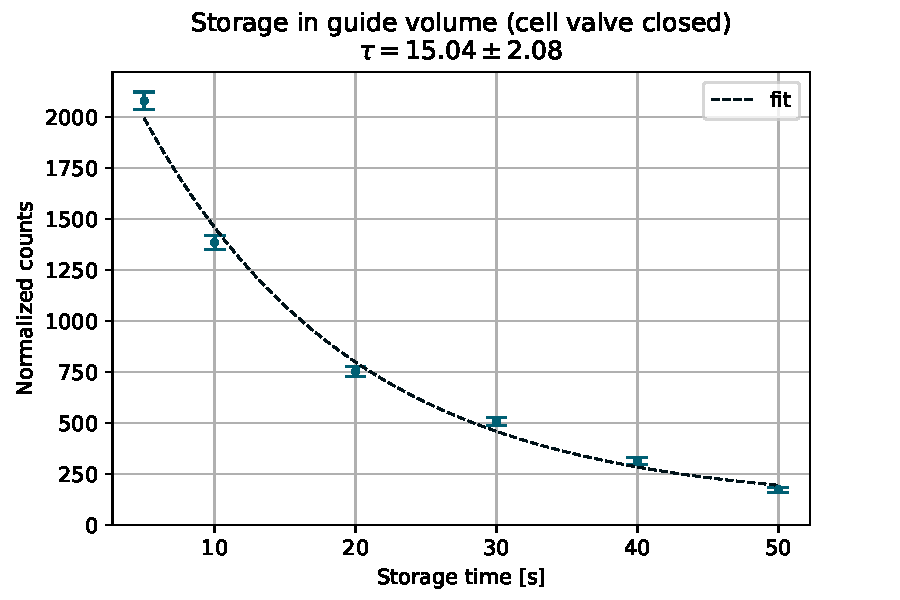
\includegraphics[width=\textwidth]{figures/store_valve_closed_fit.pdf}
  \caption{}\label{subfig:2022_guide_storage_cell_closed}
\end{subfigure}%DO NOT REMOVE THIS '%'
\begin{subfigure}{.5\textwidth}
  \centering
  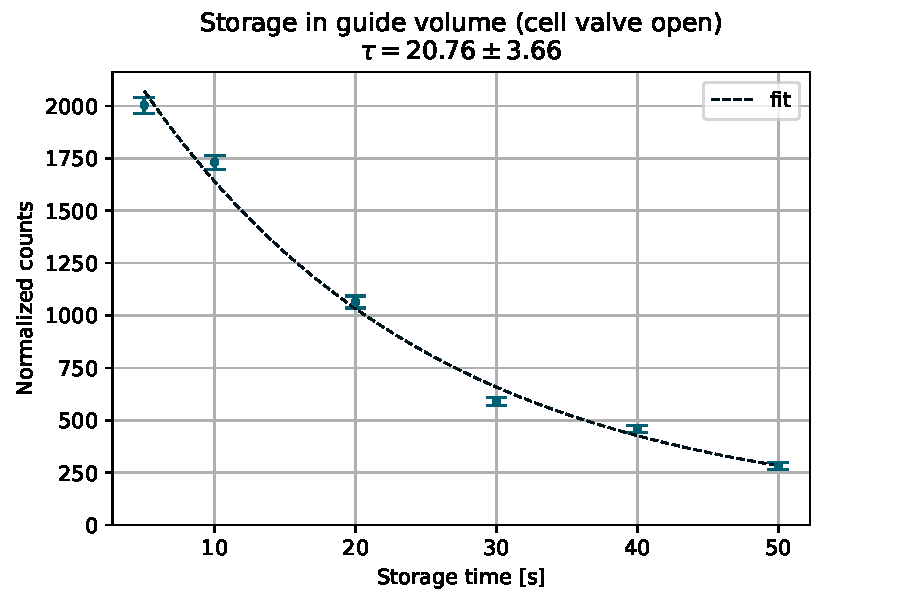
\includegraphics[width=\textwidth]{figures/store_valve_open_fit.pdf}
  \caption{}\label{subfig:2022_guide_storage_cell_open}
\end{subfigure}
\begin{subfigure}{\textwidth}
    \vspace{\baselineskip}
  \centering
  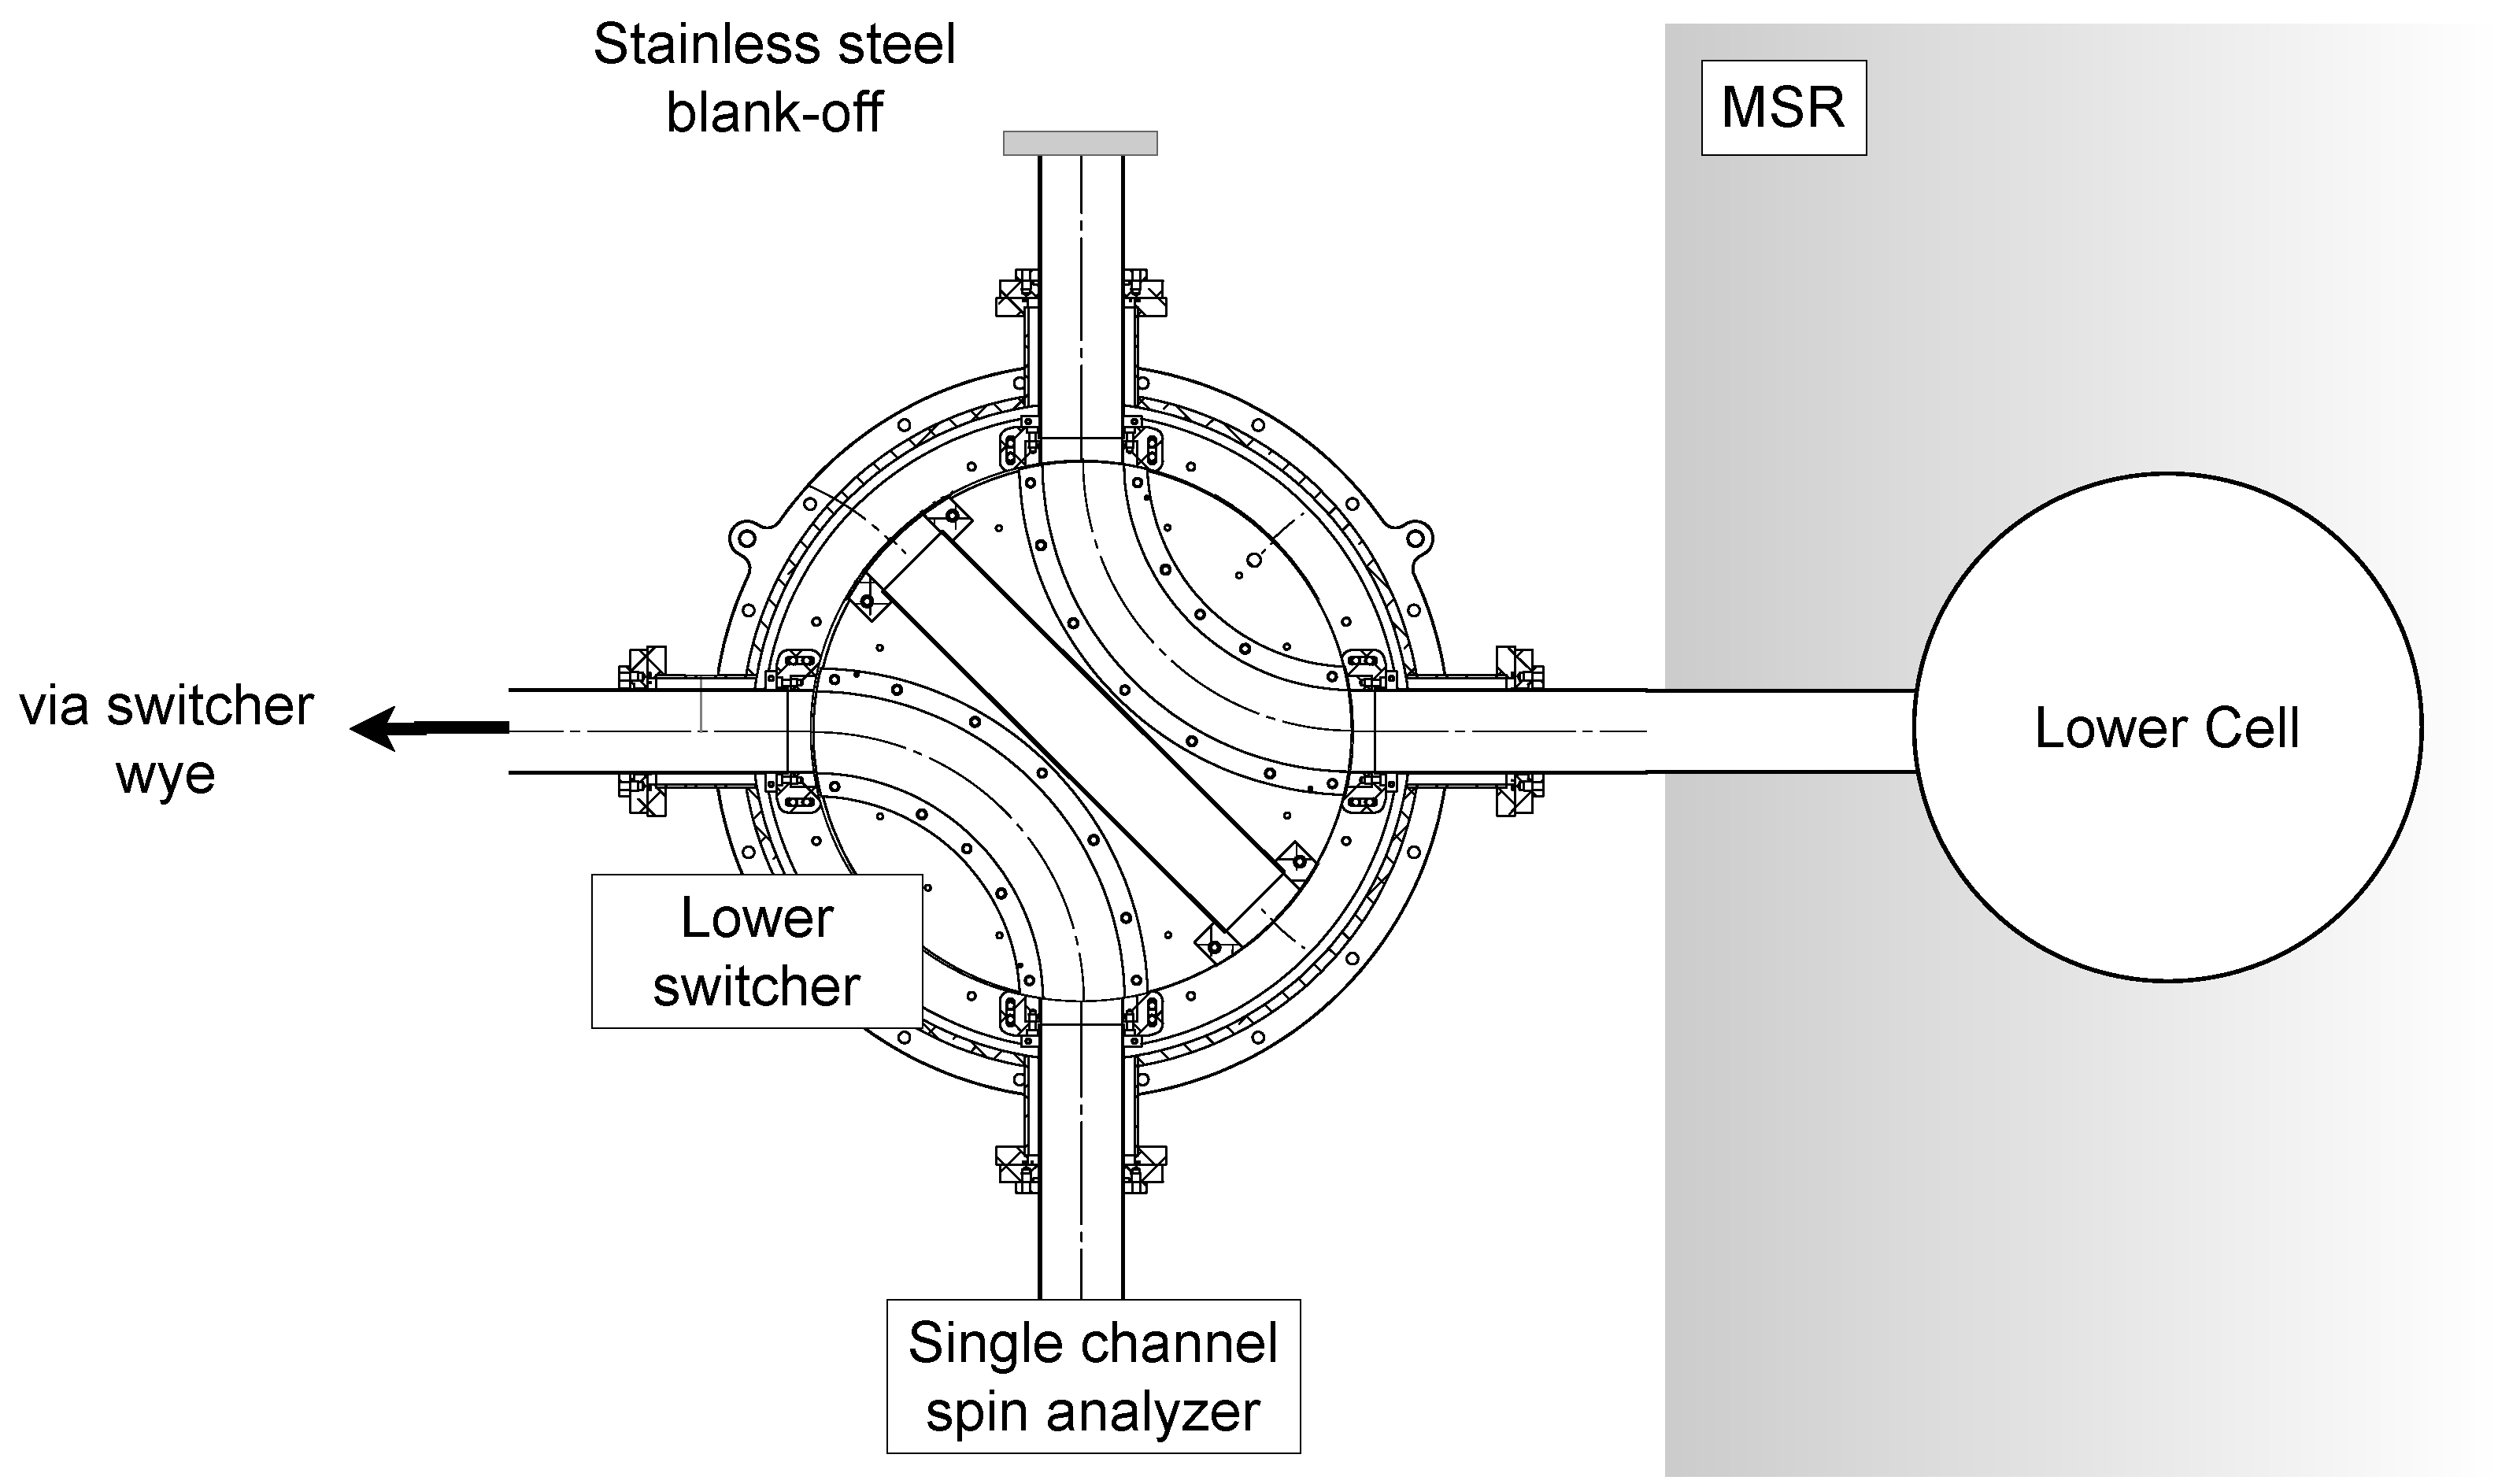
\includegraphics[width=0.8\textwidth]{figures/guide_upstream_storage.pdf}
  \caption{}\label{subfig:2022_guide_storage_schematic}
\end{subfigure}
\caption
    [Storage measurement described in Sec.~\ref{sec:guide_storage_measurement}, where UCN were stored in the guides between the lower switcher and lower cell as depicted in \textbf{(\subref{subfig:2022_guide_storage_schematic})}.]
    {Storage measurement described in Sec.~\ref{sec:guide_storage_measurement}, where UCN were stored in the guides between the lower switcher and lower cell as depicted in the top-down view \textbf{(\subref{subfig:2022_guide_storage_schematic})}. \textbf{(\subref{subfig:2022_guide_storage_cell_closed})} UCN were stored in the guide volume between a stainless steel blank-off on the switcher and the closed cell valve. \textbf{(\subref{subfig:2022_guide_storage_cell_open})} The cell valve was open, so UCN were stored in the chamber as well as the guide volume.}
\label{fig:2022_ucn_guide_storage}
\end{figure}


%%%%%%%%%%%%%%%%%%%%%%%%%%%%%%%%%%%%%%%%%%

\section{Single arm spin analyzer benchmarks}\label{sec:2022_single_arm_benchmarks}

%%%%%%%%%%%%%%%%%%%%%%%%%%%%%%%%%%%%%%%%%%


\begin{figure}
\centering
%subfigure width gets "multiplied" by includegraphics width
\begin{subfigure}{.5\textwidth} 
  \centering
  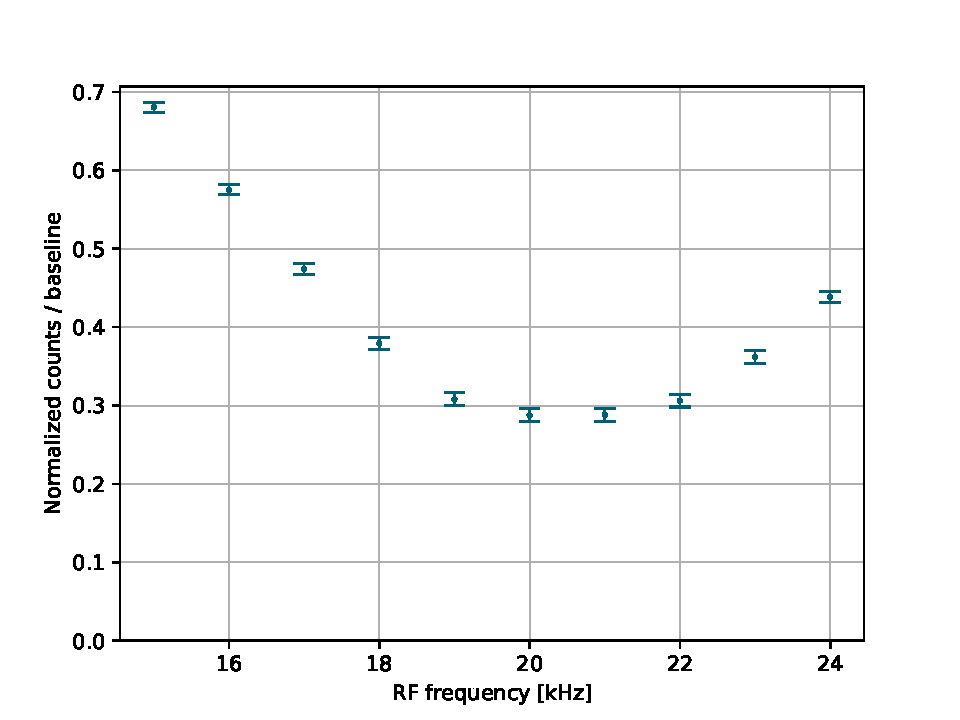
\includegraphics[width=\textwidth]{figures/2022_single_arm_spin_flip_eff.pdf}
  \caption{}\label{subfig:2022_single_arm_eff}
\end{subfigure}%DO NOT REMOVE THIS '%'
\begin{subfigure}{.5\textwidth}
  \centering
  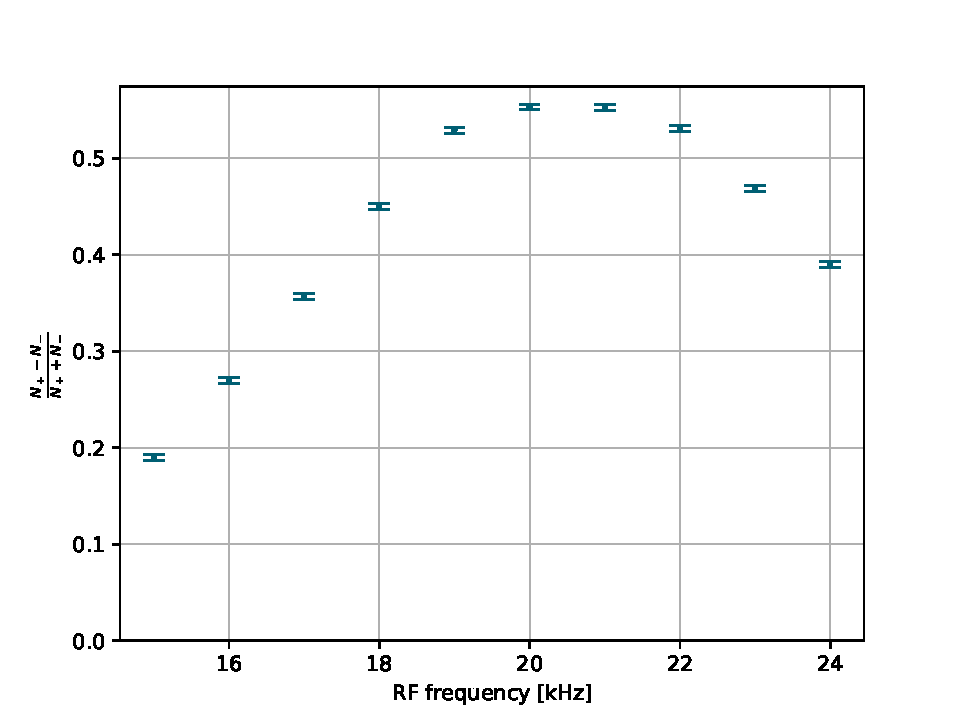
\includegraphics[width=\textwidth]{figures/2022_single_arm_spin_flip_asymmetry.pdf}
  \caption{}\label{subfig:2022_single_arm_asym}
\end{subfigure}
\caption
    [Drop detector spin flipper efficiency and spin asymmetry as function of the RF spin flipper frequency. Measured on the North beamline in 2022.]
    {\textbf{(\subref{subfig:2022_single_arm_eff})} Drop detector spin flipper efficiency as function of the RF spin flipper frequency. Measured on the North beamline in 2022. The count rate on the y-axis is normalized to the West Gate valve monitor, then divided by the baseline count rate with the spin flipper off. For $\text{Amp}=\qty{10}{Vpp}$, the minimum at \qty{20}{kHz} is 0.28. \textbf{(\subref{subfig:2022_single_arm_asym})} The same data replotted in terms of asymmetry. The asymmetry at resonance is $A=0.553(3)$}
\label{fig:2022_single_arm_asymmetry}
\end{figure}

As had become customary, a flow-through measurement (Sec.~\ref{sec:ssa_measurements}) from the source to the drop detector was used to benchmark spin asymmetry (Eq.~\ref{eq:spin_asymmetry}).  The RF was incremented every \qty{30}{s} and the counting period occurred \qty{20}{s} of each step, when the detector count rate was the most stable. As seen in Fig.~\ref{fig:2022_single_arm_asymmetry}, the asymmetry at resonance was measured to be $A\approx 0.55$. For reference, the asymmetry at resonance measured on the 2021 West beamline was $A\approx 0.15$ (Fig.~\ref{fig:2021_west_single_arm_asymmetry}), due to the  highly depolarizing roundhouse. Asymmetry measured on the North beamline in 2020 was $A\approx 0.8$ at resonance (Fig.~\ref{fig:spin_flipper_efficiency}).

As confirmation, a flow-through measurement was performed with the polarizing foil removed. The UCN rate with foil removed was compared to measurements with the foil installed (Tab.~\ref{tb:2022_drop_detector}). For these measurements, UCN the preload period was \qty{100}{s} and the upper switcher directed UCN from the wye to the beam height detector. The polarizer-installed UCN rate gave the rate of high field seekers in the system. Subtracting the polarizer-removed measurement from the polarizer-installed measurement gave the rate of low field seekers. From this, we estimated $A\approx 0.6$, which was comparable to the result from the RF-incrementing measurement (Fig.~\ref{fig:2022_single_arm_asymmetry}).

\begin{table}
    \centering
    \caption
    [North beamline UCN flow-through measurement to evaluate UCN transport in the switcher wye and switchers.]
    {North beamline UCN flow-through measurement to evaluate UCN transport in the switcher wye and switchers. Detector counts were normalized to the average West GV monitor rate. The run condition column describes whether the holding field coils for spin transport in the experiment were on, and whether the polarizer in the drop deter was installed.}\label{tb:2022_drop_detector}
    \begin{tabular}{
        l
        S[table-format = 4.0(2)]
        S[table-format = 4.0(2)]
    }
    \toprule
        {Run condition} & {Drop det.} & {Beam height det.} \\
        & {$[\unit{UCN\per s}]$} & {$[\unit{UCN\per s}]$} \\
    \midrule
        {Drop det. foil out} &  3404(24) & 3657(26)\\
        {Drop det. foil in (coils off)} & 2747(20) & 3836(28)\\
        {Drop det. foil in (coils nominal)} &  2744(20) & 3825(28)\\
    \bottomrule
    \end{tabular}
\end{table}

%%%%%%%%%%%%%%%%%%%%%%%%%%%%%%%%%%%%%%%%%%

\section{Asymmetry measurements}\label{sec:2022_asymmetry}

%%%%%%%%%%%%%%%%%%%%%%%%%%%%%%%%%%%%%%%%%%

With the flow-through asymmetry determined, spin asymmetry measurements to find the $T_1$ coherence time in the precession cell were performed. The measurements relied upon the fill-and-dump run-doublet method as shown in Figs.~\ref{subfig:ramsey2017_t1_doublet} and \ref{fig:roundhouse_rf_toggle_doublet}. Three RF toggle integration periods were used, with the RF toggling in 10--\qty{15}{s} intervals. The preload period was \qty{100}{s} and the filling period was \qty{50}{s}.

However, it was quickly realized that even the shortest storage times of \qty{30}{s} yielded an asymmetry of zero for all three integration periods. A shorter storage time could not be tested because the guide dump would bleed into the counting period, artificially inflating the number of polarized UCN. This was exemplified in a ``zero storage time'' run, where after the filling period, the switcher was immediately moved into the cell dump position. For the three integration periods in the doublet, this gave asymmetries $A_1=0.27(2)$, $A_2=-0.31(5)$, and $A_3=-0.19(3)$ .

To improve the quality of the transport field, the $B_0$ holding field was increased to as high as \qty{18}{\micro T}, and tested in both inverted and nominal orientations. The transport coils in the MSR feed throughs were also adjusted. Table~\ref{tb:t1_2022_measurements} summarizes all $B_0$ and transport coil configurations attempted, with zero asymmetry measured in all cases.


\begin{table}
\centering
\caption
[Measured asymmetry $A_i$ for various configurations of the $B_0$ and transport coils.]
{Measured asymmetry $A_i$ for various configurations of the $B_0$ and transport coils. $i$ refers to the integration period in the run doublet for which the asymmetry is calculated. The currents applied to the outer $B_0$ coils (the top 2 and bottom 2 octagons), $B_0$ coils (the middle 4 octagons), and the transport coils are listed. The filling time was \qty{50}{s} and the storage time was \qty{30}{s}.}\label{tb:t1_2022_measurements}
\begin{tabular}{
    S[table-format = 2.0]
    S
    S
    c
    S[table-format = 1.2(2)]
    S[table-format = 1.2(2)]
    S[table-format = 1.2(2)]
}
\toprule
{$\sim\vv{B_0}$} 	& {$B_0$ inner}	& {$B_0$ outer} & {Transport coils} & {$A_1$} & {$A_2$} & {$A_3$}\\
{[\unit{\micro\tesla}]} 	& {[mA]}	& {[mA]} & {out $\triangleright$ in [mA]} & {} & {} & {}\\
\midrule
1 & 3.5 & 6.3 & {$91\triangleright 23.4 \triangleright 13.5 \triangleright 10.98$} & 0.02(5) & -0.01(14) & 0.03(14) \\
18 & 56 & 100 & {$91\triangleright 70\phantom{.0} \triangleright 81\phantom{.0} \triangleright 105\phantom{.0}$} & 0.00(3) & 0.00(13) & 0.01(7) \\
-1 & -3.5 & -6.3 & {$91\triangleright 23.4 \triangleright 13.5 \triangleright 10.98$} & 0.00(3) & -0.06(11) & 0.02(5) \\
-10 & -36 & -63 & {$91\triangleright 77.2 \triangleright 89.1 \triangleright 109\phantom{.0}$} & -0.02(3) & -0.02(10) & 0.00(5) \\
\bottomrule
\end{tabular}
\end{table}


%%%%%%%%%%%%%%%%%%%%%%%%%%%%%%%%%%%%%%%%%%

\section{Discussion}

%%%%%%%%%%%%%%%%%%%%%%%%%%%%%%%%%%%%%%%%%%

We first examine UCN storage results obtained in Sec.~\ref{sec:2022_ucn_storage_measurements}. Measurements in this chapter were normalized to the average West GV monitor rate of $\approx \qty{800}{UCN \per s}$. However, normalization to the maximal West GV rate of $\qty{2000}{UCN \per s}$ still gives counts of stored UCN two orders of magnitude fewer than was previously demonstrated on the same beamline (Chap.~\ref{chap:north_beamline_paper}) with largely identical instrumentation.

One concern was whether the new cell valve was fully opened during the filling period, as the vacuum chamber prevented visual inspection. Figure~\ref{fig:2022_fill_time_sweep} seems to indicate that there is no such geometrical impedance, as increased fill time would allow the UCN gas to eventually saturate the storage volume.

Another explanation for the small amount of stored UCN is that there exists some absorber within the precession cell. However, the storage curve from Fig.~\ref{fig:2022_ucn_storage} implies that once UCN enter the precession cell that there is no such black hole. Granted, a \qty{30}{s} storage lifetime also underperforms with respect to the measurements from Chap.~\ref{chap:north_beamline_paper}, but the lifetime is also not short enough to account for a two order of magnitude reduction of stored UCN.

The next obvious UCN loss mechanism would be contaminated Cu guides in the region between the switcher and MSR, which were new additions to the beamline. However, the storage measurements in the Cu guides  (Fig.~\ref{fig:2022_ucn_guide_storage}) show that the UCN lifetime in the guides is sufficient for transport into the cell. Referring back to the earlier concern regarding cell valve actuation, storage in the Cu guide volume with the cell valve open (Fig.~\ref{subfig:2022_guide_storage_schematic}) showed a $\sim \qty{5}{s}$ improvement in storage lifetime. This is consistent with the idea that the cell valve opened sufficiently to allow UCN to propagate into the higher-lifetime cell.

We now consider the UCN spin transport measurements from Secs.~\ref{sec:2022_single_arm_benchmarks} and \ref{sec:2022_ucn_storage_measurements}. The flow-through measurements to the drop detector ($A\approx 0.55$) underperformed relative to previous measurements on the North beamline  ($A\approx 0.8$). Inspection of the magnetic field with a fluxgate along all UCN guides between the switchers and PM seemed to indicate no obvious field zeros. This seemed to be confirmed by the foil in/out measurement with the spin analyzer in Tab.~\ref{tb:2022_drop_detector}. When all holding fields were off and the polarizer was installed, the number of UCN counted (high-field seekers) was comparable to the count to when the holding fields were energized, suggesting that the ambient magnetic field in the experimental area in itself is adequate for spin transport.

As demonstrated by the measurements in Tab.~\ref{tb:t1_2022_measurements}, it is unlikely that there exists a magnetic field zero or non-adiabatic region which completely depolarizes neutrons during transport into the central apparatus. When the $B_0$ field was increased to \qty{18}{\micro T} (with a corresponding adjustment in the transport coils), it approached the magnitude of the ambient magnetic field in the experimental area $\sim\qty{50}{\micro T}$, heavily mitigating any possible adiabaticity issues. Yet, asymmetry was still measured to be zero.

It is possible that the switcher wye or some component in the beamline was highly depolarizing. We note that an additional measurement for asymmetry was performed with the upper switcher directing UCN from the wye to a moderately depolarizing SS blank-off. This gave UCN an opportunity to be depolarized on the upper switcher blank-off before traveling to the drop detector on the lower switcher, as opposed to the nominal run condition where UCN would simply be absorbed by the beam height detector. There was no significant shift demonstrated in asymmetry. Of course, it is possible that the wye is significantly more depolarizing than SS, or that there is a extremely depolarizing local surface. This is examined further using Monte Carlo simulations in Sec.~\ref{sec:switcher_height_monte_carlo}.

Solving the concerns that arise from the measurements presented in this chapter are the primary objectives of the upcoming 2023 measurement cycle. Chapter~\ref{chap:conclusion} describes steps taken to address issues with UCN storage and spin transport into the apparatus.